% SSRI poster: Toric Ideals of Non-Bipartite Graphs on Eight Vertices
% Ibrahim Rashid and Navila Zaman, Connecticut College
% 48 x 36 in landscape. Compile with pdflatex (Overleaf works as is).
\documentclass{article}

\usepackage[paperwidth=48in,paperheight=36in,left=1in,right=1in,top=0.85in,bottom=0.75in]{geometry}
\usepackage[T1]{fontenc}
\usepackage[utf8]{inputenc}
\usepackage{amsmath}
\IfFileExists{stix2.sty}{\usepackage{stix2}}{\usepackage{lmodern}}
\IfFileExists{sourcesanspro.sty}{\usepackage{sourcesanspro}}{\usepackage[scaled]{helvet}}
\usepackage{anyfontsize}
\usepackage[dvipsnames]{xcolor}
\usepackage{tikz}
\usepackage[most]{tcolorbox}
\usepackage{multicol}
\usepackage{booktabs}
\usepackage{enumitem}

% ---------- colours ----------
\definecolor{navy}{HTML}{1D3557}
\definecolor{cmblue}{HTML}{1F5FAE}
\definecolor{ncmorange}{HTML}{B8491F}
\definecolor{edgegray}{HTML}{6B7280}
\definecolor{subtext}{HTML}{374151}
\definecolor{thmbg}{HTML}{EEF2F8}
\definecolor{thmbgstrong}{HTML}{E3ECF8}
\definecolor{ivory}{HTML}{FBFAF6}
\definecolor{gridgray}{HTML}{D1D5DB}
\pagecolor{ivory}

% ---------- sizes ----------
\newcommand{\bodysize}{\fontsize{32}{44}\selectfont}
\newcommand{\labelsize}{\fontsize{34}{41}\selectfont}
\newcommand{\citesize}{\fontsize{28}{34}\selectfont}
\newcommand{\captionsize}{\fontsize{27}{37}\selectfont}
\newcommand{\tablesize}{\fontsize{30}{39}\selectfont}
\newcommand{\refsize}{\fontsize{19}{25}\selectfont}

% Four columns. \colheight (the height every column is stretched to) is
% computed after the header and footer are measured, so the poster is
% always exactly one page whatever fonts are installed.
\newlength{\colwidth}
\setlength{\colwidth}{0.2345\textwidth}
\newlength{\colheight}
\newlength{\headgap}
\setlength{\headgap}{0.5in}
\newsavebox{\headerbox}
\newsavebox{\footerbox}

\setlength{\parindent}{0pt}
\setlength{\parskip}{0.3em}
\setlength{\abovedisplayskip}{10pt}
\setlength{\belowdisplayskip}{10pt}
\setlength{\abovedisplayshortskip}{6pt}
\setlength{\belowdisplayshortskip}{10pt}

% Section heading with a navy rule underneath.
\newcommand{\sect}[1]{%
  {\sffamily\bfseries\fontsize{50}{58}\selectfont\color{navy}#1\par}%
  \vspace{4pt}{\color{navy}\hrule height 3pt}\vspace{14pt}}

% Label line at the top of a box: bold title, optional citation.
\newcommand{\boxlabel}[2]{%
  {\sffamily\bfseries\labelsize\color{navy}#1%
  \if\relax\detokenize{#2}\relax\else\ {\mdseries\citesize\color{subtext}#2}\fi\par}\vspace{6pt}}

\tcbset{posterbox/.style={enhanced,arc=10pt,left=20pt,right=20pt,top=16pt,bottom=16pt,
  before skip=0pt,after skip=0pt,fontupper=\bodysize}}
\newtcolorbox{thmbox}{posterbox,colback=thmbg,colframe=navy,boxrule=2.25pt}
\newtcolorbox{mainthm}{posterbox,colback=thmbgstrong,colframe=navy,boxrule=3pt}
\newtcolorbox{dfnbox}{posterbox,colback=white,colframe=edgegray,boxrule=2.25pt}

\setlist[itemize]{leftmargin=1.1em,label=\textbullet,itemsep=6pt,topsep=4pt,parsep=0pt}

\newcommand{\CM}{\textcolor{cmblue}{\textbf{51}}}
\newcommand{\NCM}{\textcolor{ncmorange}{\textbf{110}}}
\newcommand{\qedbox}{\rule{0.6em}{0.6em}}

\begin{document}
\pagestyle{empty}
\bodysize

% ================= HEADER =================
\sbox{\headerbox}{\begin{minipage}[t]{\textwidth}
\centering
{\fontsize{88}{100}\selectfont\bfseries\color{navy}Toric Ideals of Non-Bipartite Graphs on Eight Vertices\par}
\vspace{16pt}
{\fontsize{38}{46}\selectfont\itshape\color{subtext}When is the edge ring of a graph failing the odd cycle condition Cohen--Macaulay or Gorenstein?\par}
\vspace{16pt}
{\sffamily\fontsize{37}{44}\selectfont\bfseries Ibrahim Rashid and Navila Zaman\par}
\vspace{10pt}
{\sffamily\fontsize{27}{33}\selectfont\color{subtext}Adviser: Professor Augustine O'Keefe
  \ $\cdot$\ Department of Mathematics \ $\cdot$\ Connecticut College
  \ $\cdot$\ Summer Science Research Institute\par}
\vspace{22pt}
{\color{navy}\hrule height 6pt}
\end{minipage}}

% ================= FOOTER =================
\sbox{\footerbox}{\begin{minipage}[t]{\textwidth}
{\color{navy}\hrule height 2.25pt}
\vspace{18pt}
\begin{minipage}[t]{0.22\textwidth}
{\sffamily\bfseries\labelsize\color{navy}Acknowledgements\par}\vspace{6pt}
{\fontsize{22}{30}\selectfont We thank Professor Augustine O'Keefe for guidance throughout this
project, and the Connecticut College Summer Science Research Institute for its support.\par}
\end{minipage}%
\hfill
\begin{minipage}[t]{0.74\textwidth}
{\sffamily\bfseries\labelsize\color{navy}References\par}\vspace{6pt}
\refsize
\begin{multicols}{2}
\begin{enumerate}[label={[\arabic*]},leftmargin=2em,itemsep=2pt,topsep=0pt,parsep=0pt]
\item R.~H. Villarreal, Rees algebras of edge ideals, \emph{Comm. Algebra} 23 (1995).
\item H.~Ohsugi and T.~Hibi, Toric ideals generated by quadratic binomials, \emph{J. Algebra} 218 (1999).
\item H.~Ohsugi and T.~Hibi, Normal polytopes arising from finite graphs, \emph{J. Algebra} 207 (1998).
\item A.~Simis, W.~V. Vasconcelos and R.~H. Villarreal, The integral closure of subrings
  associated to graphs, \emph{J. Algebra} 199 (1998).
\item M.~Hochster, Rings of invariants of tori, Cohen--Macaulay rings generated by monomials, and
  polytopes, \emph{Ann. of Math.} 96 (1972).
\item R.~P. Stanley, Hilbert functions of graded algebras, \emph{Adv. Math.} 28 (1978).
\item H.~T. H\`a, S.~Kara and A.~O'Keefe, Algebraic properties of toric rings of graphs,
  arXiv:1703.08270 (2017).
\item D.~R. Grayson and M.~E. Stillman, Macaulay2; B.~D. McKay and A.~Piperno, nauty.
\end{enumerate}
\end{multicols}
\end{minipage}
\end{minipage}}

% Columns get whatever height is left after header, footer and the gaps.
\setlength{\colheight}{\dimexpr\textheight-\ht\headerbox-\dp\headerbox
  -\ht\footerbox-\dp\footerbox-\headgap-0.6in\relax}

\noindent\usebox{\headerbox}\par
\vspace{\headgap}

% ================= COLUMNS =================
\noindent
% ---------------- Column 1 ----------------
\begin{minipage}[t][\colheight][s]{\colwidth}\vspace{0pt}% anchor at top
\sect{The toric ideal of a graph}
Let $G$ be a finite simple graph with vertices $v_1,\dots,v_n$ and edges $e_1,\dots,e_m$.
Over a field $k$, define the ring map
\[
  \varphi : k[e_1,\dots,e_m] \to k[v_1,\dots,v_n], \qquad e=\{v_i,v_j\} \mapsto v_iv_j .
\]
The \textbf{toric ideal} of $G$ is $I_G=\ker\varphi$, and the \textbf{edge ring} is
$k[G]=k[e_1,\dots,e_m]/I_G$. Bipartite graphs are well understood, so we study
\textbf{connected non-bipartite} graphs; for these, $\dim k[G]=n$.

\vfill
\begin{thmbox}
\boxlabel{Theorem 1}{(Villarreal 1995; Ohsugi--Hibi 1999)}
The ideal $I_G$ is generated by the binomials
\[
  f_w = e_{i_1}e_{i_3}\cdots e_{i_{2s-1}} - e_{i_2}e_{i_4}\cdots e_{i_{2s}},
\]
one for each even closed walk $w=(e_{i_1},\dots,e_{i_{2s}})$ in $G$.
\end{thmbox}

\vfill
\sect{Example: two generators}
\begin{center}
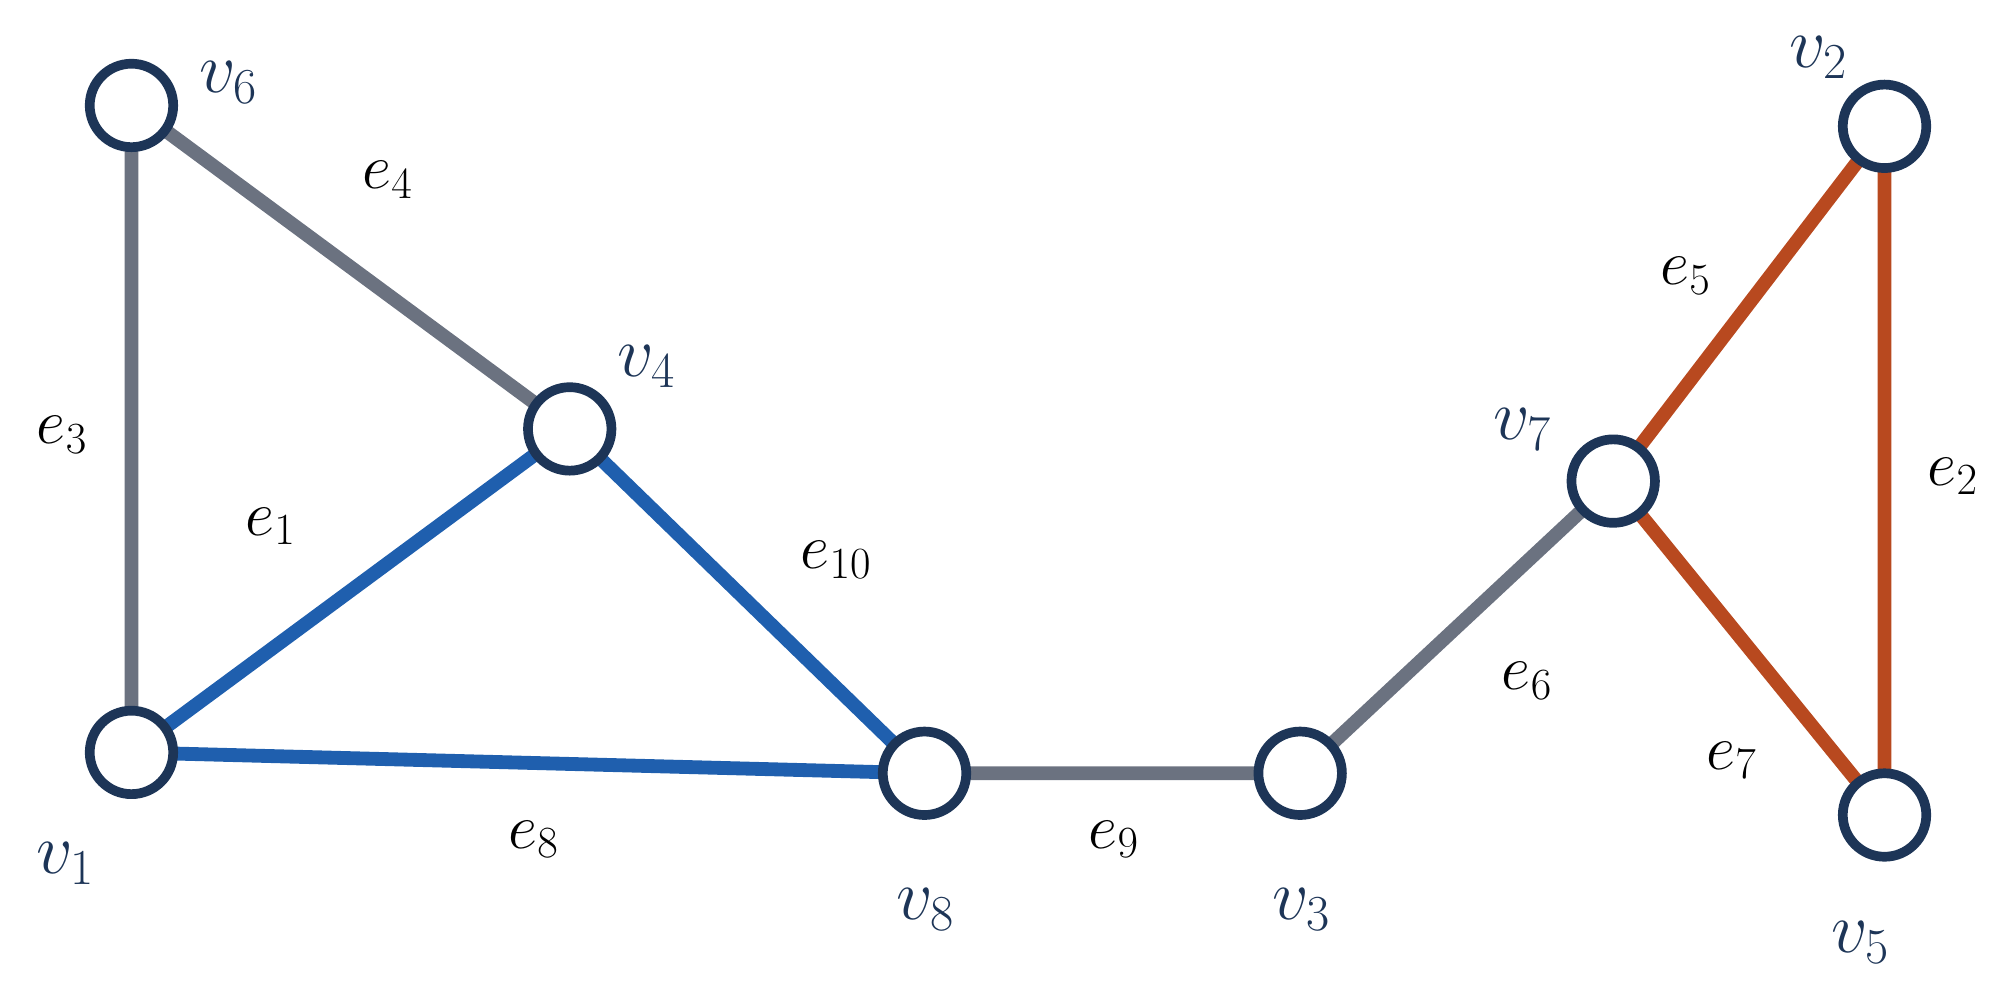
\begin{tikzpicture}[x=0.0265cm,y=-0.0265cm]
  \coordinate (v6) at (90,110);  \coordinate (v1) at (90,420);
  \coordinate (v4) at (300,265); \coordinate (v8) at (470,430);
  \coordinate (v3) at (650,430); \coordinate (v7) at (800,290);
  \coordinate (v2) at (930,120); \coordinate (v5) at (930,450);
  \begin{scope}[line width=5pt,line cap=round]
    \draw[cmblue] (v1)--(v4) (v1)--(v8) (v4)--(v8);
    \draw[ncmorange] (v2)--(v5) (v2)--(v7) (v5)--(v7);
    \draw[edgegray] (v1)--(v6) (v4)--(v6) (v3)--(v7) (v3)--(v8);
  \end{scope}
  \begin{scope}[font=\fontsize{23}{23}\selectfont]
    \node[anchor=base west] at (140,316) {$e_1$};
    \node[anchor=base west] at (946,292) {$e_2$};
    \node[anchor=base west] at (40,272)  {$e_3$};
    \node[anchor=base west] at (196,150) {$e_4$};
    \node[anchor=base west] at (818,196) {$e_5$};
    \node[anchor=base west] at (742,390) {$e_6$};
    \node[anchor=base west] at (840,428) {$e_7$};
    \node[anchor=base west] at (266,466) {$e_8$};
    \node[anchor=base west] at (544,466) {$e_9$};
    \node[anchor=base west] at (406,332) {$e_{10}$};
  \end{scope}
  \foreach \vv in {v1,v2,v3,v4,v5,v6,v7,v8}
    \filldraw[fill=white,draw=navy,line width=3.5pt] (\vv) circle (20);
  \begin{scope}[font=\fontsize{26}{26}\selectfont\bfseries,text=navy]
    \node[anchor=base west] at (118,104) {$v_6$};
    \node[anchor=base west] at (40,478)  {$v_1$};
    \node[anchor=base west] at (318,240) {$v_4$};
    \node[anchor=base west] at (452,500) {$v_8$};
    \node[anchor=base west] at (632,500) {$v_3$};
    \node[anchor=base west] at (738,270) {$v_7$};
    \node[anchor=base west] at (880,92)  {$v_2$};
    \node[anchor=base west] at (900,516) {$v_5$};
  \end{scope}
\end{tikzpicture}
\end{center}
{\captionsize\itshape\color{subtext}Graph \#2305 ($n=8$, $m=10$). The triangles
\textcolor{cmblue}{$\boldsymbol{C=v_1v_4v_8}$} and \textcolor{ncmorange}{$\boldsymbol{C'=v_2v_5v_7}$}
share no vertex and no edge joins them.\par}
\vspace{10pt}
By Theorem~1, $I_G=(g_1,g_2)$ with
\[
  g_1 = e_4e_8 - e_3e_{10}, \qquad g_2 = e_1e_5e_7e_9^2 - e_2e_6^2e_8e_{10}.
\]
$g_1$ comes from the 4-cycle $v_1v_8v_4v_6$; $g_2$ from the closed walk of length 10 around $C$,
along $v_8v_3v_7$, around $C'$ and back. Since $2=m-n$, $I_G$ is a complete intersection, and
\[
  H(k[G],t) = \frac{1+2t+2t^2+2t^3+2t^4+t^5}{(1-t)^8}.
\]
The numerator is symmetric, so $k[G]$ is Gorenstein, although $G$ fails the odd cycle condition.
\end{minipage}%
\hfill
% ---------------- Column 2 ----------------
\begin{minipage}[t][\colheight][s]{\colwidth}\vspace{0pt}% anchor at top
\begin{dfnbox}
\boxlabel{Definition (Odd cycle condition)}{}
A graph $G$ satisfies the \textbf{odd cycle condition (OCC)} if for any two vertex-disjoint
odd cycles $C$ and $C'$ of $G$, some edge of $G$ joins a vertex of $C$ to a vertex of $C'$.
A pair with no joining edge is a \textbf{separated pair}; $G$ fails OCC exactly when it has one.
\end{dfnbox}

\vfill
\begin{thmbox}
\boxlabel{Theorem 2}{(Ohsugi--Hibi 1998; Simis--Vasconcelos--Villarreal 1998)}
For a connected graph $G$, the edge ring $k[G]$ is normal if and only if $G$ satisfies the
odd cycle condition.
\end{thmbox}

\vfill
\begin{thmbox}
\boxlabel{Theorem 3}{(Hochster 1972)}
Every normal affine semigroup ring is Cohen--Macaulay.
\end{thmbox}

\vfill
\textbf{Consequence.} If $G$ satisfies OCC, then $k[G]$ is Cohen--Macaulay. The converse is
\textbf{false}: the graph in the Example fails OCC, yet $k[G]$ is Cohen--Macaulay. The open
question is which graphs \textbf{failing} OCC have Cohen--Macaulay edge rings.

\vfill
\begin{dfnbox}
\boxlabel{Definitions (Cohen--Macaulay, Hilbert series)}{}
Let $R=k[e_1,\dots,e_m]$. The ring $R/I_G$ is \textbf{Cohen--Macaulay} if
$\operatorname{depth}(R/I_G)=\dim(R/I_G)=n$. By the Auslander--Buchsbaum formula,
$\operatorname{depth}=m-\operatorname{pd}(R/I_G)$, so depth can be read off a minimal free resolution.

The Hilbert series has the reduced form
\[
  H(R/I_G,t)=\frac{h_0+h_1t+\cdots+h_st^s}{(1-t)^n},
\]
with $h$-vector $(h_0,\dots,h_s)$, $h_0=1$ and $h_1=m-n$. If $R/I_G$ is Cohen--Macaulay,
then every $h_i\ge 0$.
\end{dfnbox}

\vfill
\begin{thmbox}
\boxlabel{Theorem 4}{(Stanley 1978)}
A Cohen--Macaulay standard graded domain is Gorenstein if and only if its $h$-vector is
symmetric: $h_i=h_{s-i}$ for all $i$.
\end{thmbox}

\vfill
Since $k[G]$ is a domain, a Cohen--Macaulay edge ring with symmetric $h$-vector is Gorenstein.
Every complete intersection is Gorenstein.
\end{minipage}%
\hfill
% ---------------- Column 3 ----------------
\begin{minipage}[t][\colheight][s]{\colwidth}\vspace{0pt}% anchor at top
\begin{mainthm}
\boxlabel{Theorem 5 (Edge threshold; N.~Zaman)}{}
Let $G$ be a connected graph with $n\ge 7$ vertices and $m$ edges. If $G$ fails the odd cycle
condition, then
\[
  \mbox{\fontsize{42}{50}\selectfont$n+1 \;\le\; m \;\le\; \dfrac{n(n-1)}{2}-9,$}
\]
and every value of $m$ in this range occurs. If $n\le 6$, every connected graph satisfies OCC.
\end{mainthm}

\vfill
\sect{Proof}
\textbf{Upper bound.} Let $C$, $C'$ be a separated pair with $a$ and $b$ vertices. None of the
$ab$ pairs with one vertex in each cycle is an edge, and $a,b\ge 3$, so $G$ misses at least
$ab\ge 9$ of the $n(n-1)/2$ possible edges.

\textbf{Lower bound.} Contract $C$ and $C'$ to single vertices. The result is connected with
$n-a-b+2$ vertices, so $G$ has at least $n-a-b+1$ edges outside $C\cup C'$. Adding the $a+b$
cycle edges gives $m\ge n+1$.

\textbf{Every value occurs.} Two triangles joined by a path through the other $n-6$ vertices has
$n+1$ edges and fails OCC. Add, one at a time, every edge that does not join the two triangles:
each graph is connected and fails OCC, ending at $n(n-1)/2-9$ edges.

\textbf{Small $\boldsymbol{n}$.} Two vertex-disjoint odd cycles need at least 6 vertices; when
$n=6$ they cover every vertex, so connectivity forces an edge between them. \hfill\qedbox

\vfill
\sect{What it gives for $\boldsymbol{n=8}$}
A graph on 8 vertices can fail OCC only if $9\le m\le 19$. Every graph with 20 or more edges is
Cohen--Macaulay by Theorems 2 and 3 and needs no computation. The bound is attained at both ends:
\begin{center}
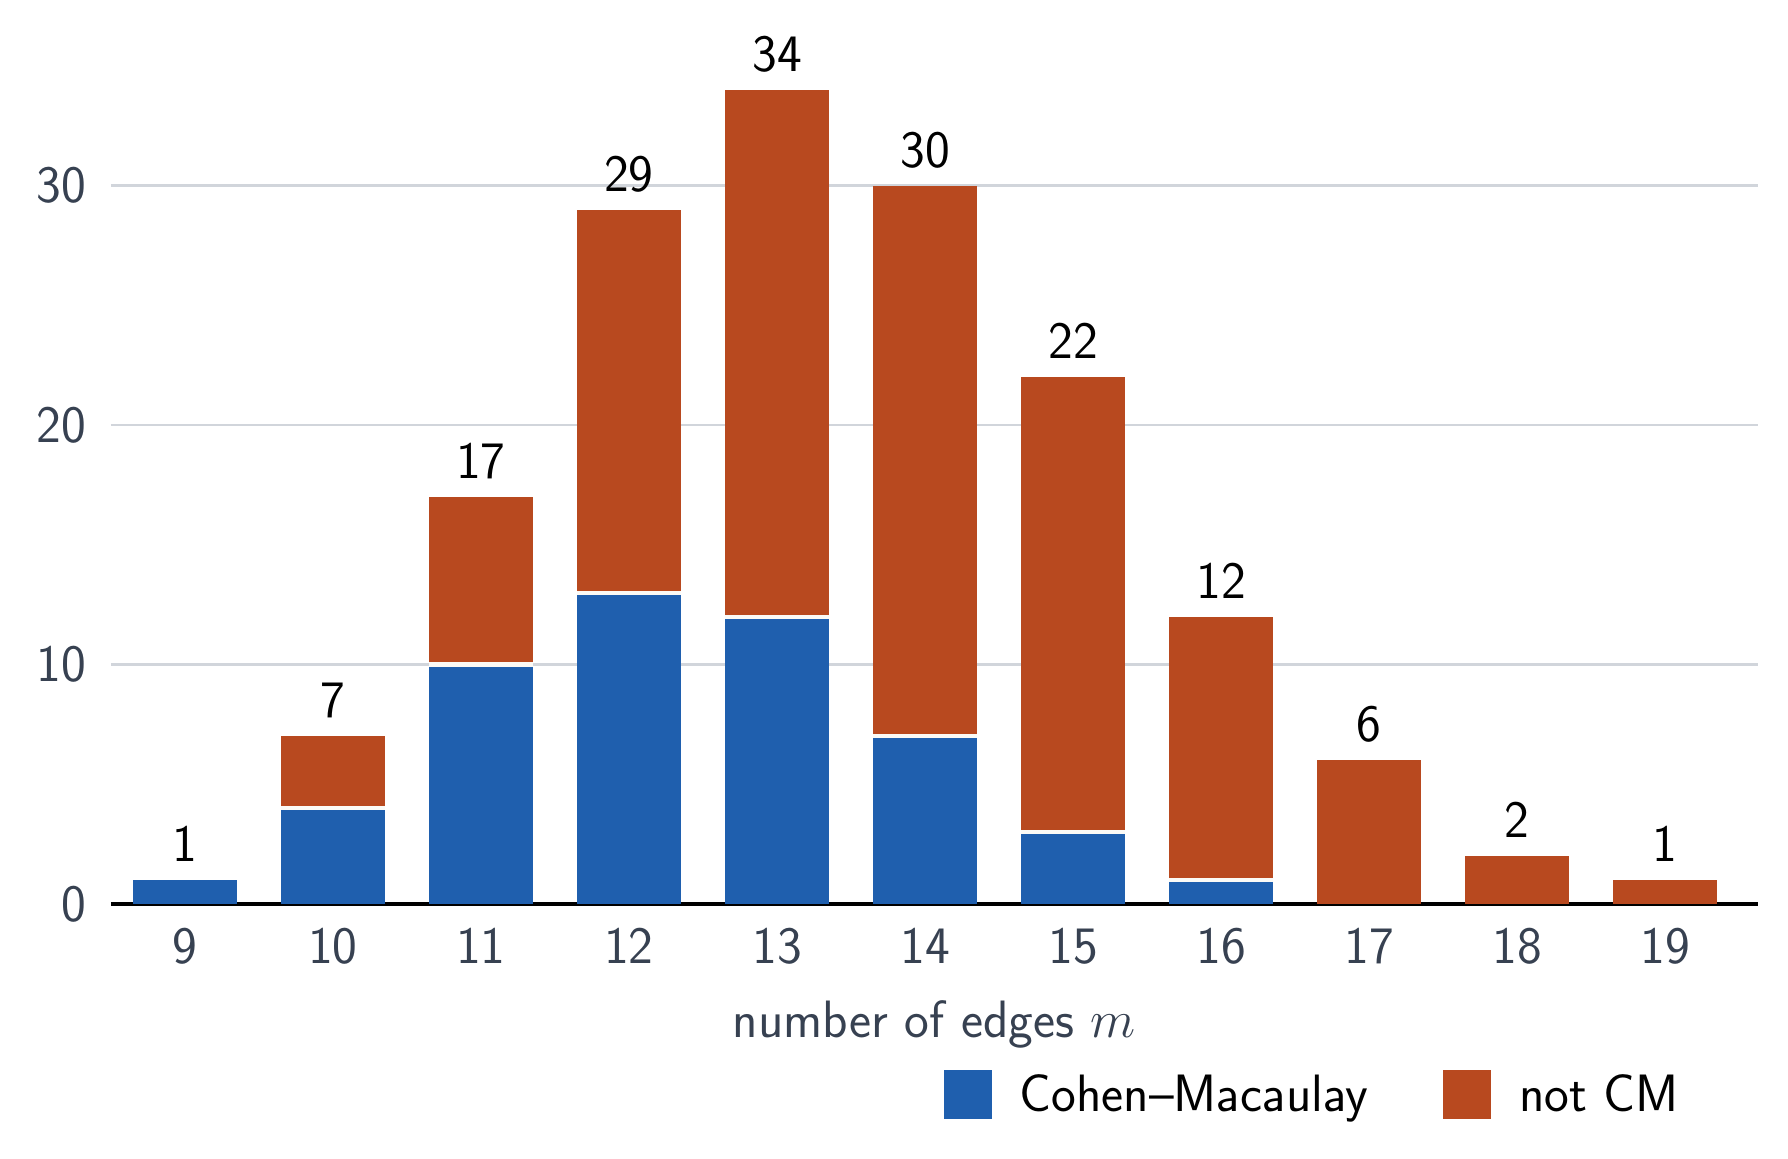
\begin{tikzpicture}[x=0.0235cm,y=-0.0235cm,font=\sffamily\fontsize{19}{22}\selectfont]
  \foreach \yy in {350.6,221.2,91.8} \draw[gridgray,line width=1pt] (70,\yy)--(960,\yy);
  \draw[black,line width=1.5pt] (70,480)--(960,480);
  \foreach \yy/\tt in {480/0,350.6/10,221.2/20,91.8/30}
    \node[anchor=east,text=subtext] at (62,\yy) {\tt};
  % bar index / edges m / CM count / not-CM count
  \foreach \bi/\bm/\bc/\bn in {0/9/1/0,1/10/4/3,2/11/10/7,3/12/13/16,4/13/12/22,5/14/7/23,
                               6/15/3/19,7/16/1/11,8/17/0/6,9/18/0/2,10/19/0/1}{
    \pgfmathsetmacro{\bx}{82+80*\bi}
    \pgfmathsetmacro{\yc}{480-12.94*\bc}
    \pgfmathsetmacro{\yn}{\yc-12.94*\bn}
    \pgfmathtruncatemacro{\tot}{\bc+\bn}
    \ifnum\bc>0 \fill[cmblue] (\bx,480) rectangle (\bx+56,\yc); \fi
    \ifnum\bn>0 \fill[ncmorange] (\bx,\yc) rectangle (\bx+56,\yn); \fi
    \ifnum\bc>0 \ifnum\bn>0 \draw[ivory,line width=1.5pt] (\bx,\yc)--(\bx+56,\yc); \fi\fi
    \node[anchor=base] at (\bx+28,\yn-10) {\tot};
    \node[anchor=base,text=subtext] at (\bx+28,512) {\bm};
  }
  \node[anchor=base,text=subtext] at (515,552) {number of edges $m$};
  \fill[cmblue] (520,570) rectangle (546,596);
  \node[anchor=base west] at (556,592) {Cohen--Macaulay};
  \fill[ncmorange] (790,570) rectangle (816,596);
  \node[anchor=base west] at (826,592) {not CM};
\end{tikzpicture}
\end{center}
{\captionsize\itshape\color{subtext}The 161 graphs on 8 vertices (connected, minimum degree
$\ge 2$) that fail OCC, by number of edges.\par}
\end{minipage}%
\hfill
% ---------------- Column 4 ----------------
\begin{minipage}[t][\colheight][s]{\colwidth}\vspace{0pt}% anchor at top
\sect{Computation}
We listed every connected graph on 8 vertices up to isomorphism (nauty, through the NautyGraphs
package of Macaulay2) and kept the non-bipartite graphs of minimum degree $\ge 2$; a leaf only adds
a free variable to $k[G]$. By Theorem 5 only $9\le m\le 19$ matters: \textbf{\color{navy}6,971}
graphs. For each, Macaulay2 computed $I_G=\ker\varphi$, $\operatorname{depth}(R/I_G)$ and the
Hilbert series. The odd cycle condition was checked separately for every graph.

\vfill
\sect{Results for $\boldsymbol{n=8}$}
{\tablesize
\begin{tabular*}{\linewidth}{@{}l@{\extracolsep{\fill}}r@{}}
\toprule
\sffamily\bfseries\color{navy} Graphs with $9\le m\le 19$ & \sffamily\bfseries\color{navy} count\\
\midrule
satisfy OCC (CM by Theorems 2, 3) & 6,810\\
fail OCC & 161\\
\quad\dots\ Cohen--Macaulay & \CM\\
\quad\dots\ not Cohen--Macaulay & \NCM\\
Gorenstein (Theorem 4) & 435\\
\bottomrule
\end{tabular*}\par}
\begin{itemize}
\item Every non-Cohen--Macaulay edge ring has depth $7=n-1$, and its $h$-vector has a negative
  entry, e.g.\ $(1,2,2,2,2,-1)$ for graph \#89.
\item 32\% of the graphs failing OCC are Cohen--Macaulay; none with $m\ge 17$ is.
\item If a separated pair lies in one 2-connected block of $G$, then $k[G]$ is not
  Cohen--Macaulay (92 of 92 graphs), consistent with H\`a--Kara--O'Keefe [7, Thm 5.1].
\item Of the 435 Gorenstein edge rings, 432 come from graphs satisfying OCC. Exactly three graphs
  fail OCC, and all three are complete intersections:
\end{itemize}
{\tablesize
\begin{tabular*}{\linewidth}{@{}l@{\extracolsep{\fill}}rll@{}}
\toprule
\sffamily\bfseries\color{navy} graph & \sffamily\bfseries\color{navy} $m$ &
\sffamily\bfseries\color{navy} generator degrees & \sffamily\bfseries\color{navy} $h$-vector\\
\midrule
\#1979 & 9  & 6       & $(1,1,1,1,1,1)$\\
\#2305 & 10 & 2, 5    & $(1,2,2,2,2,1)$\\
\#5222 & 11 & 2, 2, 4 & $(1,3,4,4,3,1)$\\
\bottomrule
\end{tabular*}\par}

\vfill
\sect{Future work}
\begin{itemize}
\item Extend the classification to 9 vertices (7,125 graphs fail OCC) and 10 vertices
  (596,940 graphs fail OCC); these computations are under way.
\item Find the structure of separated odd cycles that decides whether $k[G]$ is Cohen--Macaulay.
\item Determine when a Gorenstein edge ring of a graph failing OCC is a complete intersection.
\end{itemize}
\end{minipage}

\vfill
\noindent\usebox{\footerbox}

\end{document}
